\maketitle

\section{NEWS}

\begin{frame}
  \frametitle{new ALICE contact}
	\begin{columns}
		\begin{column}{.3\textwidth}
      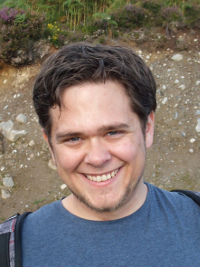
\includegraphics[width=\textwidth]{./haake_ruediger.jpeg}
		\end{column}
		\begin{column}{.7\textwidth}
      \begin{itemize}
          \item welcome to Rüdiger Haake as IML coordinator for ALICE
      \end{itemize}
		\end{column}
	\end{columns}
\end{frame}

\begin{frame}
  \frametitle{directory of people in ML for HEP}
	\begin{columns}
		\begin{column}{.3\textwidth}
			
\includegraphics[width=.9\textwidth]{./tweet.png}
		\end{column}
		\begin{column}{.7\textwidth}
			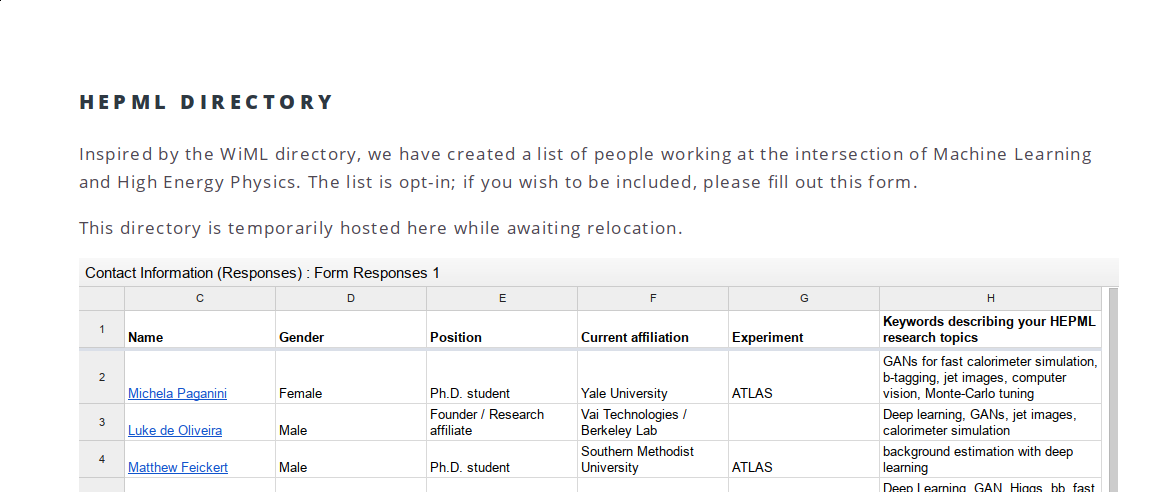
\includegraphics[width=\textwidth]{./directory.png}
		\end{column}
	\end{columns}
    \begin{itemize}
      \item field of ML in HEP is too large to know everybody
      \item[$\rightarrow$] it's easy to overlook projects when compiling summaries, recommending speakers, seeking similar projects to your own
      \item voluntary google docs form on opt-in basis
    \end{itemize}

\end{frame}

\begin{frame}
	\frametitle{today's meeting}
	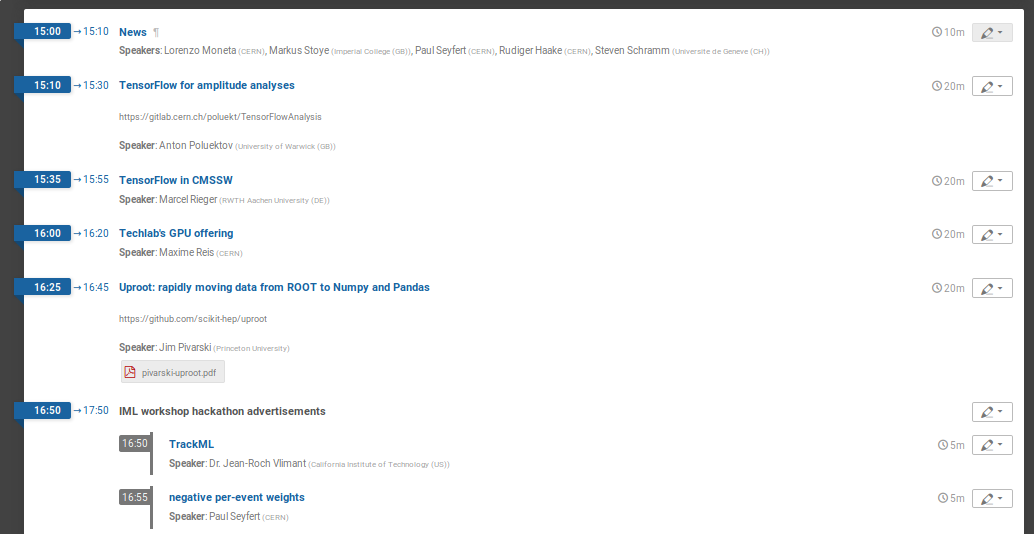
\includegraphics[width=.95\textwidth]{./agenda.png}
\end{frame}

\begin{frame}
	\frametitle{conclusion}

%	\begin{itemize}
%		\item headache ahead
%	\end{itemize}

	\vspace{.3\textheight}

	\IfFileExists{./QR2.png}{
		\footnotesize{slides (excl.\ cern logo) will appear on}

		\myhref{https://gitlab.cern.ch/pseyfert/slides-imlnews-2018-02-28}{https://gitlab.cern.ch/pseyfert/slides-imlnews-2018-02-28}
\includegraphics[width=.2\textwidth]{./QR2.png}
	}{}
\end{frame}

\appendix

